\chapter{Основные сведения об электромагнитных переходных процессах}
\section{Основные определения}
Из всего многообразия электромагнитных переходных процессов в электрической системе наиболее распространенными являются процессы, вызванные:
\begin{enumerate} 
\item
включением и отключением двигателей и других приемников электроэнергии;
\item
коротким замыканием в системе, а также повторным включением и отключением (одновременным или 
каскадным) короткозамкнутой цепи;
\item
возникновением местной несимметрии в системе (например, отключение одной фазы линии передачи);
\item
несинхронным включением синхронных машин. 
\end{enumerate}

\so{Коротким замыканием} называют всякое не предусмотренное нормальными условиями работы замыкание между фазами, а в системах с заземленными нейтралями (или четырехпроводных)~---  также замыкание одной или нескольких фаз на землю (или на нулевой провод).

В системах с незаземленными нейтралями или с нейтралями, заземленными через специальные компенсирующие устройства, замыкание одной из фаз на землю называют \so{простым замыканием}. При этом виде повреждения прохождение тока обусловлено главным образом емкостью фаз относительно земли.

При возникновении короткого замыкания в электрической системе сопротивление цепи уменьшается (степень уменьшения зависит от положения точки короткого замыкания в системе), что приводит к увеличению токов в отдельных ветвях системы по сравнению с токами нормального режима. в свою очередь это вызывает снижение напряжений в системе, которое особенно велико вблизи места короткого замыкания.

Обычно в месте замыкания образуется некоторое переходное сопротивление, состоящее из сопротивления возникшей электрической дуги и сопротивлений прочих элементов пути тока от одной фазы к другой или от фазы на землю. Электрическая дуга возникает или с самого начала происшедшего повреждения как, например, при перекрытии или пробое изоляции, или через некоторое время, когда перегорит элемент, вызвавший замыкание. При замыканиях между фазами переходное сопротивление определяется главным образом сопротивлением электрической дуги.

\begin{wrapfigure}[10]{r}{0.4\linewidth} 
	\centering
%	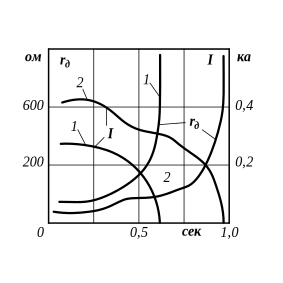
\includegraphics[width=0.5\linewidth]{1-1}
	\caption{}
	\label{fig:q}
\end{wrapfigure}

\begin{figure}
\centering
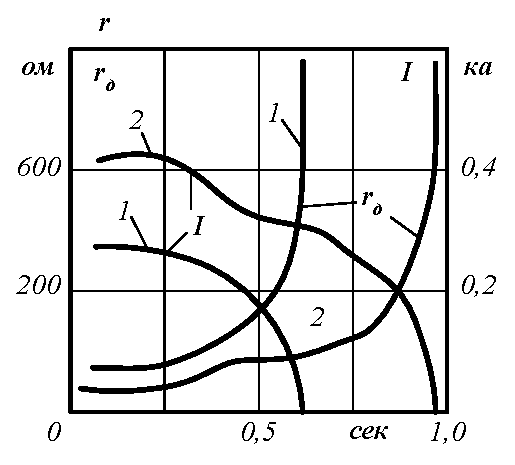
\includegraphics[width=0.7\linewidth]{a}
\caption{}
\label{fig:a}
\end{figure}


Когда токи достаточно велики (сотни ампер и более), сопротивление дуги приблизительно постоянно и по
своему характеру почти чисто активное. С уменьшением, тока и увеличением длины дуги, что имеет место в течение переходного процесса, ее сопротивление возрастает. Наглядной иллюстрацией такого изменения могут служить графики (рис. 1-1), полученные экспериментально при возникновении самопогасающих дуг на линиях
110~\textit{кв} с деревянными опорами.






